\documentclass[12pt,a4paper,oneside]{report}

\usepackage[T1]{fontenc}
\usepackage[utf8]{inputenc}
\usepackage[french]{babel}
\usepackage{newtxtext,newtxmath}            % Times (sérif 11-12 pt)
\usepackage[a4paper,margin=2cm,includefoot]{geometry} % marges 2 cm
\usepackage{graphicx,xcolor}
\graphicspath{{images/}{images/GustaveEiffelLogo/}}
\usepackage{booktabs,tabularx,longtable,array,comment}
\usepackage{amsmath}
\usepackage{listings}
\usepackage{enumitem}
\usepackage{caption}
\usepackage{float}
\usepackage{tikz}
\usetikzlibrary{arrows.meta,positioning,shapes.geometric,fit,calc}
\usepackage{pgfplots}
\pgfplotsset{compat=1.17}
\usepackage{pgfgantt}
\usepackage{csquotes}
\usepackage{fancyhdr}
\usepackage{microtype}
\usepackage{xr-hyper}
\usepackage[hidelinks]{hyperref}
\externaldocument[M-]{main}   % renvois vers le rapport principal
\usepackage{multicol,etoolbox}
\makeatletter
\patchcmd{\chapter}{\if@openright\cleardoublepage\else\clearpage\fi}{\par\bigskip}{}{}
\patchcmd{\@makechapterhead}{\vspace*{50\p@}}{\vspace*{0\p@}}{}{}
\patchcmd{\@makeschapterhead}{\vspace*{50\p@}}{\vspace*{0\p@}}{}{}
\makeatother
\usetikzlibrary{positioning, arrows.meta}
\usepackage[backend=biber,style=numeric,sorting=nyt,maxbibnames=4]{biblatex}
\addbibresource{references.bib}
\renewcommand*{\bibfont}{\small}
% Pas de date de consultation pour les articles : elle n'est gardée que pour les sites web
\DeclareSourcemap{\maps[datatype=bibtex]{\map{\pernottype{online}\step[fieldset=urldate, null]}}}

\pagestyle{fancy}\fancyhf{}\renewcommand{\headrulewidth}{0pt}
\fancyfoot[L]{\small Juvenal MALECOU NGUIMBI}\fancyfoot[R]{\small\thepage}
\fancypagestyle{plain}{\fancyhf{}\renewcommand{\headrulewidth}{0pt}%
  \fancyfoot[L]{\small Juvenal MALECOU NGUIMBI }\fancyfoot[R]{\small\thepage}}

  
\newcommand{\acompleter}[1]{\textcolor{red}{\textbf{[À compléter :} #1\textbf{]}}}
\newcommand{\averifier}[1]{\textcolor{orange!85!black}{\textbf{[À vérifier :} #1\textbf{]}}}

\setlength{\parskip}{0.4em}
\captionsetup{font=small,labelfont=bf}
\setcounter{tocdepth}{2}   % le sommaire affiche chapitres, sections, sous-sections

\begin{document}

% =====================================================================
%  PAGE DE GARDE
% =====================================================================
\begin{titlepage}
\thispagestyle{empty}
\centering

\begin{minipage}[c]{0.45\textwidth}
  \IfFileExists{images/isty.png}
    {
\includegraphics[height=2.2cm,width=\linewidth,keepaspectratio]{images/isty.png}}
    {\fbox{\parbox[c][2cm][c]{5cm}{\centering Logo ISTY}}}
\end{minipage}\hfill
\begin{minipage}[c]{0.45\textwidth}\raggedleft
  \IfFileExists{images/Dicen.png}
    {
\includegraphics[height=2.2cm,width=\linewidth,keepaspectratio]{images/Dicen.png}}
    {\fbox{\parbox[c][2cm][c]{5cm}{\centering Logo DICEN-IdF}}}
\end{minipage}

\vspace{2.2cm}
{\large Rapport de stage de fin d'année\par}
\vspace{0.3cm}
{\Large\bfseries Rapport complémentaire\par}
\vspace{0.3cm}
{\large ISTY -- IATIC4 -- Année universitaire 2025--2026\par}

\vspace{1.4cm}
\rule{\textwidth}{0.6pt}\\[0.4cm]
{\LARGE\bfseries Calculs de similarité entre exercices de programmation informatique\\[0.25cm]
\large pour la recommandation et la substitution d'exercices dans les EIAH\par}
\vspace{0.4cm}
\rule{\textwidth}{0.6pt}

\vspace{1.2cm}
{\Large Juvenal \textsc{MALECOU NGUIMBI}\par}

\vfill
\begin{tabularx}{\textwidth}{@{}>{\raggedleft\arraybackslash}p{5.2cm}X@{}}
\textbf{Structure d'accueil :} & Laboratoire DICEN-IdF -- Université Gustave Eiffel\\
\textbf{Lieu :} & Campus de Marne-la-Vallée, 5 bd Descartes, 77454 Champs-sur-Marne\\
\textbf{Dates du stage :} & du 08/06/2026 au 05/11/2026 \\
\textbf{Maître de stage :} & M. Olivier \textsc{Champalle}\\
\textbf{Tuteur pédagogique (ISTY) :} & Mme Laurence \textsc{Pilard}\\
\textbf{Confidentialité :} & OUI\\
\end{tabularx}
\end{titlepage}
\pagenumbering{roman}
\tableofcontents
\listoffigures
\listoftables
\cleardoublepage
\pagenumbering{arabic}
\renewcommand{\thechapter}{\Alph{chapter}}

% ---------- Palette et styles communs à toutes les figures -----------
\definecolor{cEIIA}{HTML}{D9822B}   % orange : EIIA
\definecolor{cTSED}{HTML}{2D6DB5}   % bleu   : TSED
\definecolor{cNCST}{HTML}{2E8B57}   % vert   : NCST
\definecolor{cNeutre}{HTML}{5A6270} % gris   : étapes communes
\definecolor{cAlerte}{HTML}{C0392B} % rouge  : différences
\definecolor{cGrille}{HTML}{BFC4CC} % gris clair : repères

\tikzset{
  >=Stealth,
  fleche/.style={->, thick, draw=cNeutre},
  etape/.style={rectangle, rounded corners=3pt, draw=#1, thick,
    fill=#1!8, font=\sffamily\small, align=center,
    minimum height=0.9cm, text width=3.0cm, inner sep=4pt},
  etape/.default=cNeutre,
  donnee/.style={rectangle, draw=#1, thick, fill=white,
    font=\sffamily\small, align=center, minimum height=0.8cm,
    text width=2.8cm, inner sep=4pt,
    double, double distance=1pt},
  donnee/.default=cNeutre,
  scorebox/.style={rectangle, rounded corners=6pt, draw=#1, very thick,
    fill=#1!18, font=\sffamily\small\bfseries, align=center,
    minimum height=0.8cm, text width=2.6cm},
  cadre/.style={draw=#1, thick, rounded corners=6pt, fill=#1!4,
    inner sep=8pt},
  titrecadre/.style={font=\sffamily\footnotesize\bfseries, text=#1,
    fill=white, inner sep=2pt},
  noeud/.style={rectangle, rounded corners=2pt, draw=#1, thick,
    fill=#1!12, font=\sffamily\scriptsize, align=center,
    minimum height=0.55cm, minimum width=1.6cm, inner sep=2pt},
  noeud/.default=cNeutre,
  code/.style={rectangle, draw=cNeutre, thick, fill=gray!6,
    rounded corners=3pt, font=\ttfamily\scriptsize, align=left,
    inner sep=6pt},
  etiq/.style={font=\sffamily\scriptsize\itshape, text=cNeutre},
}



% =====================================================================
% Chapitre : Ma proposition (version mise à jour : NCST normalisé,
% appariement naïf ordonné et interface Streamlit)
% ---------------------------------------------------------------------
% Packages requis dans le préambule du rapport :
%   \usepackage[T1]{fontenc}
%   \usepackage[utf8]{inputenc}
%   \usepackage[french]{babel}
%   \usepackage{amsmath,amssymb}
%   \usepackage{booktabs,tabularx,array}
%   \usepackage{xcolor}
%   \usepackage{listings}
%   \usepackage{tikz}
%   \usetikzlibrary{positioning,arrows.meta,fit,calc,shapes.misc,backgrounds,babel}
%   (la bibliothèque TikZ « babel » est indispensable avec babel français)
% =====================================================================

% ---------- Couleurs et styles communs ----------
\definecolor{eiiacol}{RGB}{230,120,20}
\definecolor{tsedcol}{RGB}{30,90,180}
\definecolor{ncstcol}{RGB}{30,140,70}
\definecolor{uicol}{RGB}{120,60,160}
\definecolor{graycol}{RGB}{110,110,110}

\tikzset{
  box/.style={draw, rounded corners=2pt, align=center, font=\small,
    minimum height=0.8cm, inner sep=4pt, fill=white},
  frame/.style={draw, rounded corners=4pt, inner sep=8pt, thick},
  flow/.style={-{Stealth[length=2.2mm]}, thick},
  nnode/.style={draw=ncstcol, fill=ncstcol!10, rounded corners=1.5pt,
    font=\ttfamily\scriptsize, inner sep=2.5pt, minimum height=0.42cm,
    anchor=west},
  nlink/.style={draw=ncstcol!70!black, thin},
  elab/.style={font=\ttfamily\tiny, text=graycol, fill=white, inner sep=0.8pt},
  lvl/.style={font=\ttfamily\scriptsize, anchor=west},
}

\lstdefinestyle{pyncst}{
  language=Python, basicstyle=\ttfamily\small, keywordstyle=\color{tsedcol}\bfseries,
  commentstyle=\color{graycol}, frame=single, rulecolor=\color{ncstcol},
  framesep=4pt, xleftmargin=6pt, xrightmargin=6pt, showstringspaces=false,
  columns=fullflexible, keepspaces=true, backgroundcolor=\color{ncstcol!4}
}

\chapter*{Avant-propos}
\addcontentsline{toc}{chapter}{Avant-propos}
Ce document complète le rapport de stage principal. Il rassemble les
éléments techniques qui allègent la lecture de ce dernier : le panorama
détaillé des méthodes de la littérature, les pistes explorées puis
écartées, les règles précises de construction des représentations, le
fonctionnement de l'interface et l'analyse détaillée des résultats sur les
variantes contrôlées. Les numéros de chapitres, de figures et de tableaux
qui commencent par un chiffre (par exemple « figure 4.2 ») renvoient au
rapport principal ; ceux qui commencent par une lettre renvoient au présent
document.

\chapter{Panorama détaillé des outils et méthodes}
\label{chap:outils}

Les travaux présentés dans le rapport principal (section~\ref{M-sec:domaines}) ne comparent pas tous les exercices à la
même échelle. Selon l'objectif poursuivi, la comparaison peut porter sur le
texte de l'énoncé, les concepts pédagogiques associés, les traces d'activité,
la forme du programme, ses dépendances ou encore son comportement à
l'exécution. Les outils employés sont donc différents, mais ils suivent
généralement une chaîne commune modélisée par la
figure~\ref{fig:pipeline_generique}.

Cette chaîne répond à quatre questions : quelles données sont disponibles,
sous quelle représentation sont-elles transformées, comment la proximité
est-elle calculée et à quelle fonction de l'EIAH le résultat est-il destiné ?
Cette distinction est importante pour comparer les méthodes. Deux approches
peuvent utiliser une même mesure, par exemple la similarité cosinus, tout en
comparant des objets différents : deux énoncés, deux corrections ou un énoncé
et une correction. À l'inverse, deux approches peuvent partir du même code,
mais extraire des informations différentes : l'une peut retenir la structure
syntaxique, une autre les dépendances entre instructions et une troisième les
propriétés observées à l'exécution. Ce chapitre présente ces familles dans cet ordre ; leur
synthèse et leurs limites sont discutées dans le rapport principal.


\iffalse
Les difficultés et les limites propres à chaque famille
seront discutées dans la section suivante.
\fi




\begin{figure}[H]
    \centering
    \begin{tikzpicture}[
        >=Stealth,
        node distance=1.3cm and 1.8cm,
        boite/.style={draw=blue!80!black, thick, rounded corners, fill=blue!5,
            align=center, text width=6.0cm, minimum height=1.55cm,
            font=\normalsize, inner sep=7pt},
        fleche/.style={->, line width=1.2pt, color=gray!80!black}
    ]
    
    \node[boite] (source) {\textbf{1. Données sources}\\(Énoncé, Code, Traces)};
    \node[boite, right=of source] (repr) {\textbf{2. Représentation}\\(Vecteurs, AST, Graphes)};
    \node[boite, below=of source] (sim) {\textbf{3. Mesure et calcul}\\(Cosinus, TED, Isomorphisme)};
    \node[boite, right=of sim] (exploit) {\textbf{4. Exploitation (EIAH)}\\(Recommandation, Rétroaction)};
    
    \draw[fleche] (source) -- (repr);
    \draw[fleche] (repr) -- (sim);
    \draw[fleche] (sim) -- (exploit);
    
    \end{tikzpicture}
    \caption{Étapes communes aux méthodes de comparaison d'exercices pédagogiques}
    \label{fig:pipeline_generique}
\end{figure}

\paragraph{Représentation textuelle et traitement automatique du langage.}

La première famille traite l'énoncé comme un \textbf{document textuel}.
Une étape de prétraitement nettoie le texte et le segmente en unités
(mots ou fragments de mots) : c'est la \emph{tokenisation}, ou découpage en
lexèmes, qui peut se faire de plusieurs façons. Selon la méthode, les mots
jugés peu informatifs sont ensuite supprimés (\emph{stop word removal}).
Les approches lexicales représentent alors chaque énoncé par un vecteur de
fréquences, par exemple avec la pondération TF--IDF : chaque texte devient
un vecteur orienté dans un espace, et deux textes sont d'autant plus proches
que leurs vecteurs le sont. La proximité entre deux exercices est calculée
à l'aide d'une distance ou d'une similarité entre vecteurs, le plus
souvent la similarité cosinus.

Les méthodes fondées sur les représentations distribuées vont au-delà du
simple partage de mots. Un modèle de type Word2Vec ou FastText transforme les
mots en vecteurs appris à partir de leur contexte. Pour l'appariement
d'exercices avec des compétences, Tian \emph{et al.} combinent ainsi des
représentations lexicales produites par FastText avec une extraction de
concepts clés, puis utilisent un classifieur pour estimer les
\emph{knowledge components} associés à un exercice
\cite{tian_2022}. Cette combinaison permet de rapprocher le vocabulaire
employé dans l'énoncé de concepts pédagogiques explicites.

Les modèles Transformers proposent une représentation contextualisée des
mots et des phrases. BERT et Sentence-BERT produisent des vecteurs qui
intègrent le contexte d'apparition des termes ; Sentence-BERT est notamment
conçu pour comparer efficacement des phrases ou des paragraphes
\cite{reimers_sentence-bert_2019}. Dans un système de recherche d'exercices, chaque énoncé
peut ainsi être transformé en un vecteur, puis comparé à ceux des
autres énoncés. Les résultats peuvent servir à la recherche de ressources
voisines ou être combinés avec des informations pédagogiques et des traces
d'apprentissage \cite{liu_2018,pelanek_2020}.

\paragraph{Concepts pédagogiques, annotations et traces d'apprentissage.}

Une deuxième famille ne cherche pas d'abord une ressemblance de surface :
elle représente l'exercice par les compétences ou les notions nécessaires à
sa résolution. Ces notions peuvent être définies par des experts sous la
forme de \emph{knowledge components}, de concepts algorithmiques ou de
compétences du langage. L'outil de comparaison devient alors un système
d'annotation ou de classification. Il reçoit le texte de l'exercice, ses
métadonnées ou sa correction, et prédit un ensemble de concepts associés.
Les scores de proximité sont ensuite calculés à partir de l'intersection,
de la pondération ou de la distance entre ces ensembles de concepts
\cite{tian_2022,hosseini_2017}.

Les systèmes de recommandation peuvent compléter ces informations par les
traces d'utilisation de la plateforme : nombre de tentatives, temps passé,
taux de réussite, ordre des exercices ou types d'erreurs rencontrées. Des
méthodes de filtrage ou de classement exploitent ces données pour proposer
un exercice similaire à un apprenant ou pour retrouver, dans une banque,
des activités présentant des caractéristiques proches
\cite{liu_2018}. La similarité n'est alors plus seulement une propriété du
contenu : elle dépend aussi des parcours et des comportements observés.

\paragraph{Tests dynamiques et métriques de programme.}

Dans l'évaluation des exercices de programmation, une autre méthode consiste
à exécuter les solutions. Le programme soumis et la correction de référence
sont lancés sur un ensemble de tests unitaires ou de tests de propriétés.
Les sorties obtenues, les exceptions et les temps d'exécution sont comparés.
Cette approche fournit une information comportementale directe et constitue
la base de nombreux correcteurs automatiques. La revue systématique de
Messer \emph{et al.} montre que les outils d'évaluation combinent souvent
tests dynamiques, analyse statique et, dans certains cas, apprentissage
automatique pour produire une note ou un retour à l'étudiant
\cite{messer_2024}.

Les outils peuvent aussi extraire des métriques statiques : nombre de lignes,
nombre de fonctions, profondeur d'imbrication, complexité cyclomatique,
nombre de variables ou fréquence de certaines constructions. Ces valeurs
forment un vecteur numérique qui peut être comparé par une distance euclidienne,
une distance normalisée ou un modèle de régression. Dans les approches
hybrides, les métriques statiques sont associées aux résultats des tests afin
de tenir compte à la fois du comportement observé et de l'organisation du
code \cite{messer_2024,vujosevic-janicic_software_2013}.

\paragraph{Arbres syntaxiques, distances d'édition et rétroactions.}

Les approches syntaxiques commencent par l'analyse du code source à l'aide
d'un parseur. Celui-ci vérifie la grammaire du langage et construit un arbre
de syntaxe abstraite, ou AST. Chaque nœud représente une construction du
programme, par exemple une affectation, une condition, une boucle, un appel
de fonction ou une opération. L'AST supprime une partie des détails de mise
en forme tout en conservant l'organisation syntaxique du programme.

Les AST peuvent être comparés directement. Les méthodes de détection de
clones de Baxter \emph{et al.} utilisent cette représentation pour repérer
des fragments identiques ou presque identiques dans des programmes
\cite{baxter_clone_1998}. Pour comparer deux arbres de tailles différentes, la
distance d'édition entre arbres compte les opérations nécessaires pour
transformer le premier arbre en second : insertion, suppression et
substitution de nœuds. L'algorithme de Zhang et Shasha fournit une méthode
classique pour calculer cette distance sur des arbres ordonnés
\cite{zhang_simple_1989}.

Dans une application à la similarité de code, la distance brute est souvent
normalisée par la taille des arbres afin d'obtenir un score comparable entre
des programmes courts et longs. Une phase de normalisation peut également
remplacer les noms de variables, les valeurs littérales ou certaines
variantes syntaxiques par des catégories communes. L'objectif est de
comparer l'ossature de la solution plutôt que ses détails accidentels. Les
travaux consacrés à l'évaluation de la similarité par AST étudient ainsi la
normalisation de l'arbre et l'impact de la distance d'édition sur le score
final \cite{song_revisiting_2024}.

La même représentation peut également servir à produire une rétroaction
pédagogique. Dans AlgoPython, Jolivet \emph{et al.} comparent l'AST d'une
production étudiante avec celui d'une solution de référence afin de localiser
les différences et de décider d'une rétroaction épistémique adaptée au profil
de l'apprenant \cite{jolivet_modelisation_2025}. L'AST joue alors le rôle
d'une représentation intermédiaire : les différences entre les arbres sont
transformées en informations compréhensibles et exploitables dans le parcours
d'apprentissage. La similarité sert donc à caractériser l'écart entre une
production et une référence, et pas uniquement à classer des exercices.

\paragraph{Graphes de flot, dépendances et graphes sémantiques.}

L'AST décrit principalement la construction syntaxique du code. Pour
représenter plus explicitement son fonctionnement, les chercheurs utilisent
différents graphes complémentaires. Un graphe de flot de contrôle
(\emph{Control Flow Graph}, CFG) représente les chemins possibles
d'exécution : ses nœuds correspondent à des instructions ou à des blocs, et
ses arêtes indiquent les transitions possibles entre ces éléments.

Les relations entre les instructions peuvent également être représentées par
des graphes de dépendances. Un graphe de dépendances de données
(\emph{Data Dependence Graph}, DDG) relie une instruction qui définit une
valeur aux instructions qui utilisent cette valeur. Il permet ainsi de
représenter les dépendances entre variables, affectations et expressions. Un
graphe de dépendances de contrôle décrit quant à lui l'influence d'une
condition ou d'une structure de contrôle sur l'exécution d'une instruction.
Le graphe de dépendances de programme (\emph{Program Dependence Graph},
PDG) combine généralement ces deux informations : il regroupe les
dépendances de données et les dépendances de contrôle au niveau d'une
fonction ou d'un programme \cite{xiang_graph_2024,reddy_graph-based_2025}.

À une échelle plus large, le graphe de dépendances système
(\emph{System Dependence Graph}, SDG) étend le PDG à plusieurs fonctions en
représentant notamment les relations entre les appels de fonctions, leurs
paramètres et leurs valeurs de retour. D'autres représentations associent
plusieurs types d'informations dans un même modèle. C'est notamment le cas
du graphe de propriétés du code (\emph{Code Property Graph}, CPG), qui
combine généralement l'AST, le CFG et les dépendances de données et de
contrôle. Des outils tels que Joern exploitent ce type de représentation
pour effectuer des analyses statiques et rechercher des propriétés
structurelles ou sémantiques du code.

Les graphes peuvent être comparés par leurs nœuds, leurs arêtes, leurs
chemins ou leurs sous-structures. On peut calculer une distance d'édition de
graphes, rechercher des sous-graphes communs ou extraire des caractéristiques
structurelles avant d'appliquer une mesure vectorielle. Vujošević-Janičić
\emph{et al.} combinent ainsi vérification logicielle et analyse de graphes
pour l'évaluation automatique de travaux étudiants
\cite{vujosevic-janicic_software_2013}. Xiang \emph{et al.} utilisent
également des représentations fondées sur les dépendances du code pour
comparer une solution étudiante à une solution de référence dans le cadre
d'exercices de programmation \cite{xiang_graph_2024}.

La sélection du graphe dépend du compromis recherché entre richesse de la
représentation, précision de l'analyse et coût de calcul. L'AST est
relativement compact et facile à extraire. Le CFG décrit l'organisation du
flot d'exécution, tandis que le DDG et le PDG rendent explicites les
relations entre les calculs et les variables. Le SDG permet d'étudier les
interactions entre fonctions, alors qu'un CPG rassemble plusieurs de ces
dimensions dans une représentation unifiée. L'étude comparative de Paiva
\emph{et al.} examine plusieurs représentations de graphes sémantiques et
compare notamment leur coût et leur pouvoir descriptif
\cite{paiva_comparing_2024}. Les travaux de synthèse sur la similarité
sémantique des exercices regroupent ces méthodes avec les approches fondées
sur les graphes de contrôle et de dépendances
\cite{reddy_graph-based_2025}.

Ces représentations peuvent également être utilisées pour produire une
rétroaction à partir d'une analyse statique du code. La comparaison des PDG,
des DDG ou des CPG permet par exemple de localiser une dépendance manquante,
une structure de contrôle inattendue ou une utilisation incorrecte d'une
variable. Paiva \emph{et al.} comparent plusieurs représentations
graphiques afin d'évaluer leur richesse, leur coût et leur capacité à
supporter une rétroaction automatique \cite{paiva_comparing_2024}. Les
graphes ne servent donc pas uniquement à calculer un score de similarité :
ils peuvent aussi rendre les différences entre une solution étudiante et une
référence plus explicables.

\paragraph{Représentations vectorielles et modèles appris.}

Les méthodes d'apprentissage automatique transforment le texte ou le code en
vecteurs denses, appelés \emph{embeddings}. Une première stratégie consiste
à extraire des chemins dans l'AST et à apprendre leur représentation. Le
modèle code2vec, par exemple, agrège des chemins AST pour produire un vecteur
de code \cite{alon_2019} ; code2seq exploite également les chemins de l'arbre
dans un modèle séquence-à-séquence \cite{alon_code2seq_2019}.

Les modèles pré-entraînés spécialisés dans le code constituent une autre
famille. CodeBERT apprend conjointement à partir de code et de langage
naturel, ce qui permet de rapprocher une implémentation de sa documentation
ou de comparer des fragments dans un espace commun \cite{feng_2020}. À la
différence d'un modèle qui ne considère que la séquence de tokens,
GraphCodeBERT introduit le flot de données entre variables et des objectifs
d'apprentissage sensibles à cette structure. Il utilise notamment une
attention guidée par le graphe pour intégrer les relations de données dans
la représentation \cite{guo_2021}.

\paragraph{Évaluation vectorielle par CodeBERT : spécialisation et limites.}

Face aux limites des règles explicites fondées sur les tags ou les AST, nous
avons également envisagé l'utilisation d'un modèle d'apprentissage profond
spécialisé dans le code : CodeBERT. Celui-ci produit des plongements
vectoriels du code, appris à partir de tâches de compréhension et de
génération de programmes. Son évaluation s'appuie notamment sur plusieurs
objectifs associés au génie logiciel :

\begin{itemize}
    \item la \textbf{détection de clones}, qui consiste à déterminer si deux
    fragments de code sont des clones selon un apprentissage binaire ;
    \item le \textbf{code search}, qui vise à retrouver un fragment de code
    à partir d'une intention exprimée en langage naturel ;
    \item le \textbf{refinement}, qui cherche à améliorer la qualité ou
    l'efficacité d'un code sans en modifier la fonction, par exemple en
    transformant une boucle naïve en compréhension de liste ;
    \item la \textbf{translation}, qui consiste à convertir
    automatiquement un programme d'un langage vers un autre, par exemple de
    Python vers Java, au moyen d'une architecture séquence--séquence.
\end{itemize}

Ces tâches rendent les représentations de CodeBERT particulièrement
pertinentes pour la recherche de similarité fonctionnelle entre programmes.
Elles ne suffisent toutefois pas à mesurer la substituabilité pédagogique.
En effet, un modèle ajusté pour distinguer des clones ou pour rapprocher des
solutions fonctionnellement similaires tend à produire un signal de
proximité binaire ou fortement corrélé à la similarité de résolution. Il ne
permet donc pas nécessairement de distinguer un exercice dont la résolution
est trop proche, et qui rendrait sa réalisation peu utile à un étudiant ayant
déjà réussi le premier, d'un exercice partageant le même thème tout en
exigeant un effort cognitif nouveau. Les poids du modèle ne sont pas alignés
sur des critères de compétences pédagogiques : un score élevé peut ainsi
traduire une proximité fonctionnelle sans constituer une preuve de
substituabilité dans un parcours d'apprentissage.

Pour comparer deux exercices, ces modèles peuvent produire un vecteur pour
chaque énoncé, correction ou paire énoncé--code. La proximité est ensuite
calculée par similarité cosinus, distance euclidienne ou score appris. Les
modèles siamois et l'apprentissage contrastif rapprochent les représentations
de deux objets considérés comme similaires et éloignent les autres exemples.
Dans le domaine des exercices multimodaux, BCRNet combine texte et images
avec une perte contrastive et un mécanisme d'appariement texte--image afin
d'apprendre une représentation utilisable pour la recherche et la
recommandation \cite{mu_2023}.

\paragraph{Vérification formelle et comparaison comportementale.}

Les méthodes formelles ne se limitent pas à mesurer une proximité : elles
cherchent à démontrer une propriété du programme. Le code peut être traduit
en une représentation logique, puis soumis à un vérificateur ou à un
solveur. Pour prouver l'équivalence de deux programmes, on peut utiliser la
réécriture des boucles en fonctions récursives, l'induction fonctionnelle et
un solveur de satisfaisabilité modulo théories (SMT). Dans ses travaux sur
l'équivalence de programmes, Milovančević s'appuie sur le vérificateur
Stainless et sur des preuves d'induction fonctionnelle pour comparer des
programmes candidats à des programmes de référence
\cite{milovancevic_automated_nodate}.

Dans un contexte de cours, la vérification formelle peut compléter les tests
et distinguer des solutions qui ont le même comportement sur les entrées
testées mais qui reposent sur des structures de résolution différentes.
L'expérience de Vafeiadis \emph{et al.} illustre l'utilisation d'un
vérificateur d'équivalence conjointement avec une infrastructure de
correction par tests \cite{vafeiadis_formal_2025}. Cette famille produit donc
une information très forte sur le programme, mais elle répond à une question
de correction ou d'équivalence qui n'est pas exactement celle de la
substituabilité pédagogique.




\chapter{Pistes explorées et écartées}
\label{chap:pistes}

La définition du pipeline retenu est le résultat de plusieurs explorations
préliminaires. L'objectif de ces essais n'était pas seulement d'obtenir le
meilleur score possible, mais aussi d'identifier des représentations
compatibles avec les données disponibles, suffisamment interprétables et
réutilisables sur un corpus d'exercices potentiellement hétérogène. Plusieurs
pistes ont ainsi été étudiées sans être retenues comme méthodes principales.

\paragraph{Étiquetage par mots-clés et modèles génératifs.}

Une première piste, explorée dans les travaux préliminaires d'Adel
\textsc{Ziani}, consistait à caractériser chaque exercice au moyen d'étiquettes
conceptuelles telles que \emph{boucle}, \emph{récursivité}, \emph{liste} ou
\emph{condition}. L'extraction de ces étiquettes a notamment été testée à
l'aide de modèles de langage génératifs (LLM), afin d'identifier
automatiquement les notions mobilisées par les corrections
\cite{ziani_detection_2025}.

Cette approche s'est toutefois révélée difficile à stabiliser. Les réponses
des LLM peuvent varier selon la formulation de la requête et le contexte
fourni ; les étiquettes produites et les regroupements obtenus ne sont donc
pas nécessairement reproductibles ni cohérents d'une exécution à l'autre.
Par ailleurs, une liste fermée de mots-clés impose un vocabulaire défini à
l'avance. Si une correction mobilise une structure ou une notion absente de
cette liste, cette information n'est pas représentée. Dans une représentation
vectorielle fondée uniquement sur ces étiquettes, l'exercice peut alors
présenter un vecteur nul ou incomplet, ce qui fausse le calcul de similarité.
Les LLM ont donc été conservés comme piste exploratoire, mais ils ne
constituent pas la base du pipeline retenu.

\paragraph{Extraction de motifs syntaxiques avec Tree-sitter.}

Au cours du présent stage, une autre piste a consisté à remplacer cet
étiquetage génératif par une extraction déterministe de motifs syntaxiques.
L'outil Tree-sitter a été utilisé pour analyser les corrections et rechercher
explicitement des structures telles que les conditions, les boucles, les
appels de fonctions ou les retours. L'objectif n'était plus de comparer
directement les arbres entiers, mais de produire automatiquement des
caractéristiques structurelles à partir du squelette du code.

Cette approche permet de rendre l'extraction reproductible et indépendante
des variations de réponse d'un modèle génératif. Elle reste cependant limitée
par les motifs définis dans le programme d'analyse. Le parseur ne peut
identifier que les structures qui ont été anticipées et codées dans les règles
d'extraction ; une démarche algorithmique non prévue est ignorée ou réduite à
une représentation incomplète. Elle reproduit ainsi, sous une forme plus
déterministe, le biais d'une liste fermée de tags.



\paragraph{Comparaison des énoncés par TF--IDF et SBERT.}

Une première piste consistait à comparer directement les textes des énoncés.
Cette approche présente l'avantage de partir d'une information immédiatement
disponible, sans nécessiter l'analyse du code source. La représentation TF--IDF
fournit ainsi un point de référence simple et rapide. Pour chaque énoncé, elle
attribue à chaque terme un poids qui dépend de deux éléments : la fréquence du
terme dans l'énoncé et sa rareté dans l'ensemble du corpus. Un mot très fréquent
dans un document mais peu présent dans les autres énoncés reçoit donc un poids
important, tandis qu'un mot présent partout contribue peu à différencier les
exercices. Chaque énoncé est ainsi transformé en un vecteur numérique, puis les
vecteurs de deux exercices sont comparés à l'aide de la similarité cosinus.
Cette mesure évalue si les deux vecteurs pointent dans des directions proches,
ce qui revient principalement à mesurer le partage de termes importants.

Des représentations produites par SBERT  ont également
été envisagées afin de dépasser cette comparaison fondée sur les mots. Le
modèle transforme chaque phrase, ou chaque énoncé, en un vecteur dense appris à
partir du contexte des mots. Deux formulations différentes peuvent ainsi être
rapprochées lorsqu'elles expriment une idée similaire, même si elles ne
partagent pas exactement le même vocabulaire. La similarité entre les vecteurs
SBERT est elle aussi généralement calculée avec la similarité cosinus, mais le
score porte alors sur une représentation sémantique et non plus seulement sur
la fréquence des termes.

Ces deux méthodes ne décrivent cependant pas directement la manière dont le
programme doit être construit. TF--IDF reste sensible aux mots employés dans
l'énoncé, tandis que SBERT peut rapprocher des phrases dont le sens général est
semblable sans distinguer les structures de contrôle ou les algorithmes
attendus. Elles ont donc été utilisées comme premières approximations de la
proximité thématique.

Ces essais ont fourni un signal de proximité thématique, mais ce signal ne
permet pas de caractériser suffisamment la démarche de résolution. Des
énoncés peuvent employer des termes différents tout en demandant des
algorithmes proches. Inversement, deux énoncés peuvent partager un vocabulaire
lié aux listes, aux boucles ou aux fonctions tout en nécessitant des solutions
structurellement différentes. Ces méthodes ont donc été conservées comme
éléments exploratoires ou comme informations complémentaires possibles, mais
elles n'ont pas été retenues comme source principale de similarité.

La dynamique entre ces deux méthodes est illustrée par la figure~\ref{fig:tfidf_sbert}, qui compare directement les scores de similarité TF--IDF et SBERT pour l'ensemble des paires d'énoncés du corpus.

\begin{figure}[htbp]
\centering
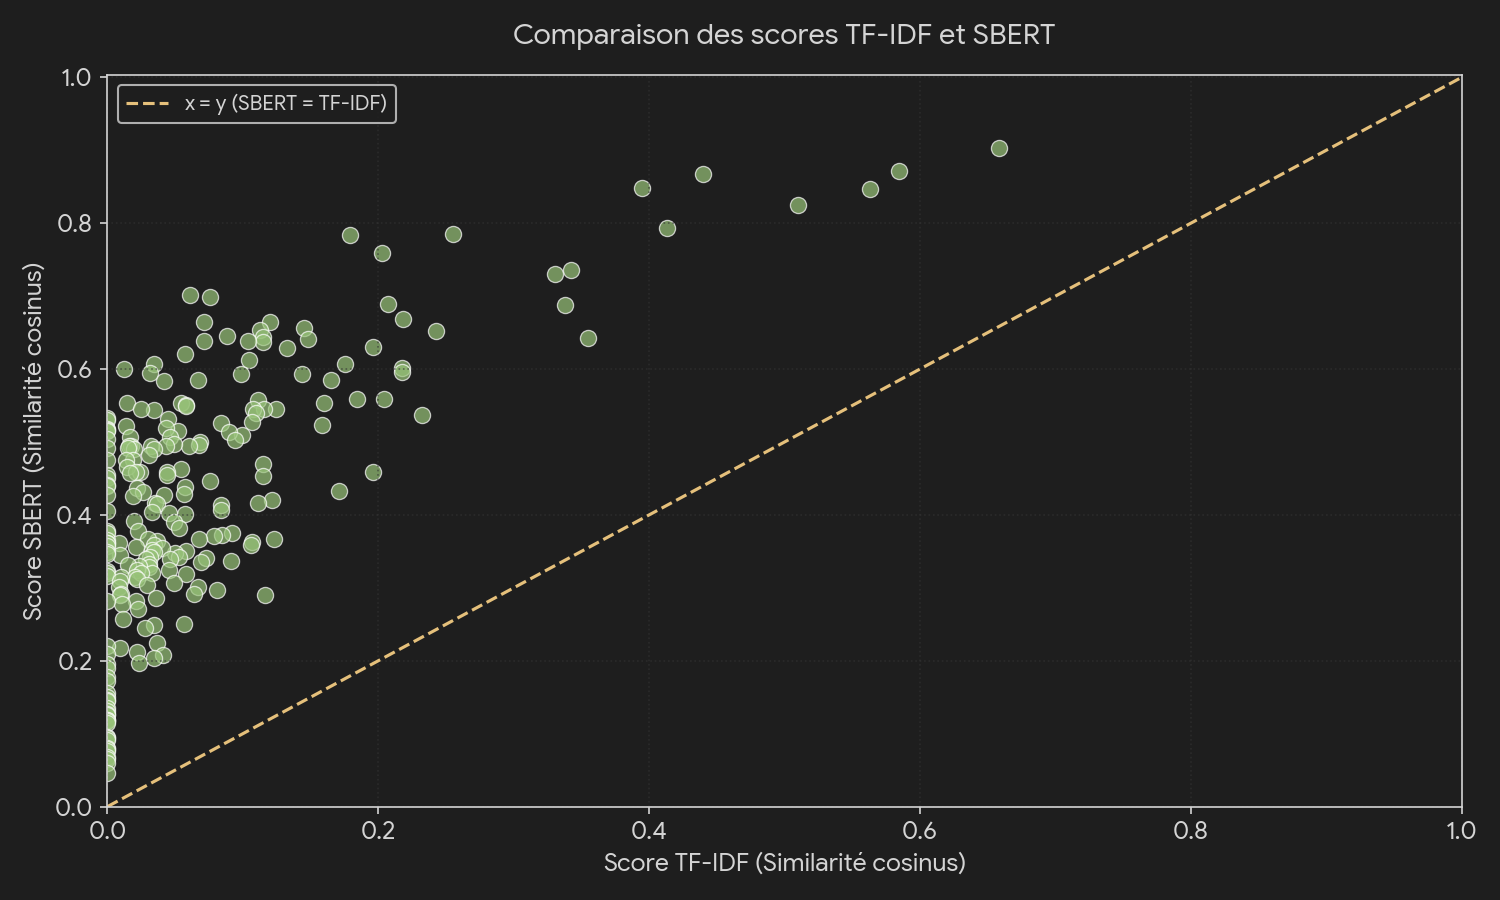
\includegraphics[width=0.8\textwidth]{TDF-IDF_SBERT.png}
\caption{Comparaison des scores de similarité cosinus TF--IDF et SBERT pour l'ensemble des paires d'énoncés. La ligne pointillée représente l'égalité des scores.}
\label{fig:tfidf_sbert}
\end{figure}

L'analyse de cette distribution confirme empiriquement les limites de ces approches textuelles. La quasi-totalité des points se situe au-dessus de la ligne d'égalité, démontrant que SBERT attribue des scores systématiquement plus élevés (moyenne de 0,42) que TF--IDF (moyenne de 0,07). L'importante dispersion verticale sur la gauche du graphique montre la capacité de SBERT à rapprocher des énoncés partageant une sémantique commune mais aucun vocabulaire (TF--IDF proche de 0). Cependant, l'absence de regroupements (clusters) distincts prouve que ces scores thématiques peinent à segmenter finement les exercices selon leur démarche de résolution algorithmique.

Pour illustrer concrètement ces limites, nous pouvons examiner un  cas représentatif tiré de notre corpus, mettant en évidence les \og illusions \fg{} lexicales :

\paragraph{Exemple : l'illusion lexicale (TF--IDF élevé, structures différentes).}
\begin{itemize}
\item \textit{Énoncé A :} \og Écrire un programme qui demande une somme cible entre 2 et 12, puis affiche toutes les combinaisons possibles de deux dés à six faces donnant cette somme. Afficher aussi le nombre total de combinaisons. \fg{}
\item \textit{Énoncé B :} \og Écrire un programme qui demande à l'utilisateur un nombre de dés (entre 1 et 8) et une somme cible. Le programme doit afficher combien de combinaisons de résultats permettent d'obtenir cette somme avec des dés à six faces. \fg{}
\end{itemize}

Pour cette paire, les deux méthodes accordent des scores très élevés (TF--IDF = 0,65 ; SBERT = 0,90) en raison du fort
champ lexical partagé (dés, somme, combinaisons). Pourtant, le premier énoncé se résout par de simples boucles imbriquées
fixes, tandis que le second requiert une approche récursive ou une gestion dynamique pour un nombre variable de dés.
Les métriques textuelles échouent à capturer cette rupture de complexité structurelle.

\paragraph{Comparaison de séquences de jetons (stratégie de JPlag).}

JPlag compare les programmes en deux étapes \cite{prechelt_finding_nodate}.
Chaque programme est d'abord transformé en une suite de jetons : les noms de
variables et les valeurs sont effacés, seuls restent des éléments comme
\og début de boucle \fg{} ou \og affectation \fg{}. Les deux suites sont
ensuite comparées en cherchant les plus longs morceaux identiques qu'elles
ont en commun (\emph{Greedy String Tiling}).

La première étape rejoint notre démarche : la normalisation de l'AST efface
elle aussi les noms et les valeurs. La seconde ne correspond pas à notre
objectif. JPlag cherche de longs passages identiques, signe qu'un programme
a été recopié. Or deux exercices substituables ne sont pas des copies : ils
suivent la même démarche avec une écriture qui peut varier. Remplacer une
boucle \texttt{for} par une boucle \texttt{while} ou changer l'ordre de deux
instructions suffit à couper la suite de jetons en petits morceaux, alors
que la démarche est inchangée. De plus, une suite de jetons est
\og à plat \fg{} : elle ne dit pas quelle instruction se trouve à
l'intérieur de quelle boucle, alors que cette imbrication décrit justement
la démarche de résolution. Nous avons donc gardé l'idée de normalisation,
mais remplacé la comparaison de séquences par une comparaison d'arbres.


 

\paragraph{Graphes de dépendances et modélisations hybrides (CFG, PDG, CPG, CSSG).}

Pour dépasser la rigidité topologique des Arbres Syntaxiques Abstraits (AST), la modélisation des flux d'exécution a été explorée afin de capturer l'essence sémantique du code. Contrairement à un AST qui décrit la forme syntaxique stricte, les graphes de flot de contrôle (CFG) modélisent les différents chemins d'exécution possibles, tandis que les graphes de dépendances de données (DDG) et de programme (PDG) explicitent les relations entre la définition d'une variable et ses utilisations ultérieures. Ces graphes présentent l'avantage majeur de rester stables même si un étudiant réordonne des instructions indépendantes ou modifie la syntaxe de surface.

Pour obtenir une représentation absolue, des approches hybrides telles que les CPG (Code Property Graphs) ou les CSSG (Code Syntax and Semantics Graphs) ont été étudiées. Le modèle CSSG, par exemple, fusionne l'AST, le CFG et le PDG en une structure de données unique, capturant simultanément la syntaxe et la sémantique d'exécution.

Cependant, cette piste s'est heurtée à un obstacle technique majeur lors de la phase de comparaison. Évaluer la similarité exacte entre deux graphes aussi riches et denses nécessite de calculer des distances d'édition de graphes (Graph Edit Distance) ou de rechercher des isomorphismes de sous-graphes. Ces opérations mathématiques étant d'une complexité algorithmique NP-difficile, le temps de calcul explose de manière exponentielle. Cette approche s'est donc révélée inapplicable pour évaluer et comparer à grande échelle un corpus important d'exercices en temps raisonnable. Elle demeure une perspective théorique d'enrichissement, mais a été écartée du pipeline principal.

\paragraph{Modèles appris et embeddings de code (CodeBERT et GraphCodeBERT).}

Face aux limites combinatoires des graphes, l'utilisation de modèles de langage pré-entraînés spécialisés dans le code source a été envisagée pour projeter les programmes dans un espace vectoriel dense (embeddings). Le modèle CodeBERT s'appuie sur une architecture Transformer entraînée conjointement sur du langage naturel et du code, tandis que son évolution, GraphCodeBERT, y intègre la structure du flux de données (data flow) pour mieux saisir la logique algorithmique sous-jacente.

Si ces modèles excellent dans la représentation globale du code, ils présentent une limite conceptuelle fondamentale par rapport à notre objectif. Ces architectures sont pré-entraînées sur des tâches de génie logiciel rudimentaires, telles que la recherche de code (Code Search) ou la détection binaire de clones (déterminer si un code A est le plagiat d'un code B). Par conséquent, les espaces vectoriels qu'ils génèrent sont optimisés pour la similarité fonctionnelle stricte, et échouent à mesurer la notion de substituabilité pédagogique.

Ces modèles ne parviennent pas à différencier un exercice dont la démarche de résolution est sémantiquement identique (et donc inutile à recommander à un étudiant qui maîtrise déjà le concept) d'un exercice partageant une thématique proche mais exigeant une structure de contrôle inédite (et donc pertinent pour la progression). Pour devenir exploitables dans un Environnement Informatique d'Apprentissage Humain (EIAH), ces modèles nécessiteraient un réentraînement profond (fine-tuning) sur de larges volumes de paires d'exercices annotées par des enseignants selon leur valeur d'apprentissage, une ressource actuellement indisponible à l'échelle requise. Ils ont donc été écartés au profit de représentations plus interprétables et ne nécessitant pas d'apprentissage préalable.

\paragraph{Apprentissage contrastif pour la similarité pédagogique.}

Pour lever l'obstacle des paires annotées, une méthode d'apprentissage
contrastif a été proposée. Elle s'inspire de BCRNet \cite{mu_2023} et des
travaux sur l'apprentissage contrastif d'images, de phrases et de code
\cite{chen_simclr_2020,gao_simcse_2021,jain_contracode_2021}. L'objectif est
d'apprendre une représentation vectorielle unique de chaque exercice, qui
réunit l'énoncé et la correction, sans recourir à des paires étiquetées
manuellement.

Pour chaque exercice, on génère deux \emph{vues} qui conservent le même
contenu pédagogique et le même comportement du code, mais dont la forme
diffère. Ces deux vues forment une \textbf{paire positive} que le modèle
apprend à rapprocher dans l'espace de représentation. Les vues des autres
exercices du lot d'entraînement forment des \textbf{paires négatives} que le
modèle apprend à éloigner, au moyen de la perte InfoNCE \cite{oord_infonce_2018}.
Le signal d'apprentissage vient donc uniquement de la structure du problème :
deux vues d'un même exercice doivent être proches. La méthode reposait sur
trois éléments :
\begin{itemize}
  \item \textbf{les vues de l'énoncé}, obtenues par \emph{dropout} appliqué à
        l'encodeur de texte, à la manière de SimCSE \cite{gao_simcse_2021}.
        Le masquage de mots utilisé par BCRNet a été écarté, car il fournit
        un signal faible à un modèle déjà pré-entraîné par masquage
        (\emph{masked language modeling}) ;
  \item \textbf{les vues de la correction}, obtenues par des transformations
        qui préservent la sémantique et que la littérature a déjà validées
        \cite{jain_contracode_2021,bui_corder_2021} : renommage des variables,
        suppression des commentaires, reformatage et réordonnancement
        d'instructions indépendantes ;
  \item \textbf{une fusion multimodale}, sur le modèle de BCRNet : l'énoncé
        et le code sont encodés séparément, leurs vecteurs sont concaténés,
        puis projetés dans un espace latent commun qui fournit un plongement
        unique par exercice.
\end{itemize}

Cette piste n'a pas été retenue, car elle repose sur deux types de paires
et nous ne pouvions en construire qu'un seul. Les paires positives sont faciles
à obtenir : il suffit de créer des variantes bruitées d'un même exercice.
Les paires négatives, en revanche, doivent être de vrais exemples
d'exercices \emph{non similaires}. Or, dans notre situation de démarrage à
froid, aucune annotation ne permet de savoir quels exercices sont différents.
Prendre simplement les autres exercices du lot comme négatifs reviendrait à
supposer qu'ils ne se ressemblent pas, alors que c'est justement ce que l'on
cherche à mesurer : deux exercices du corpus peuvent très bien être
similaires. Sans négatifs fiables, le modèle ne peut pas apprendre
correctement la notion de similarité.

L'idée des variantes bruitées a toutefois été conservée sous une autre
forme : les variantes contrôlées du chapitre~\ref{M-chap:resultats} du rapport principal ne servent
pas à entraîner un modèle, mais à \emph{vérifier} le comportement des mesures.

\paragraph{Fusion immédiate des signaux.}

Enfin, une fusion directe de toutes les mesures disponibles aurait pu produire
un score unique combinant texte, métriques, AST et structures de contrôle.
Cette solution aurait simplifié le classement des paires, mais elle aurait
également masqué la contribution de chaque représentation. Elle aurait en
outre nécessité de fixer des pondérations sans disposer d'une vérité terrain
ou de jugements d'enseignants pour les apprendre.


\chapter{Détails de l'AST normalisé}
\label{chap:ast}

\section{Conversion du CST en AST simplifié}
\label{sec:conversion_ast}


La conversion parcourt les nœuds nommés du CST et associe à chaque type
Tree-sitter un type de l'AST interne au moyen d'une table de correspondance.
Les nœuds anonymes (mots-clés, ponctuation) ne sont pas conservés, à
l'exception des opérateurs, qui sont recopiés comme valeur du nœud
(\texttt{BINARY\_OP(+)}, \texttt{COMPARE(==)}, \texttt{UNARY\_OP(not)}).

Une table de correspondance ne couvre jamais toute la grammaire du
langage, et le traitement des types absents influe directement sur les
mesures. Leur attribuer un label générique commun, par exemple
\texttt{UNKNOWN}, rendrait identiques des constructions sans rapport : pour
le TSED, une compréhension de liste, une négation \texttt{not}, une tranche
\texttt{l[1:3]} ou une définition de classe deviendraient des nœuds
substituables à coût nul. Sur le corpus GitHub, ces constructions sont
fréquentes : on y compte notamment 23 compréhensions de liste, 13
définitions de classe, 8 négations et 7 tranches.

Plutôt que de chercher à couvrir toute la grammaire de Python, la conversion
applique quatre règles simples (tableau~\ref{tab:kind_map}) :
\begin{itemize}
  \item \textbf{types ajoutés à la table} : une construction ne reçoit son
        propre type que si elle traduit un choix de résolution. Par exemple,
        filtrer une liste avec une boucle \texttt{for} ou avec la
        compréhension \texttt{[x for x in liste if x \% 2 == 0]} sont deux
        démarches différentes : la compréhension reçoit donc le type
        \texttt{LIST\_COMP}, pour que les mesures puissent les distinguer.
        Son \texttt{for} et son \texttt{if} sont en revanche typés
        \texttt{FOR} et \texttt{IF}, comme une boucle et un test ordinaires,
        puisqu'ils réalisent eux aussi une itération et une sélection. Le
        même raisonnement s'applique à la négation (\texttt{not x}), aux
        tranches (\texttt{l[1:]}) et aux classes. Les tuples
        (\texttt{a, b}) et les paires clé-valeur (\texttt{k: v}) reçoivent
        aussi un type, afin que les valeurs qu'ils regroupent ne se mélangent
        pas avec les nœuds voisins ;
  \item \textbf{feuilles} : une chaîne de caractères et un import ne gardent
        aucun enfant, quel que soit leur découpage interne par l'analyseur.
        Toute instruction qui commence par \texttt{import} ou
        \texttt{from}, quelle que soit sa forme (alias, nom pointé, import
        relatif ou \texttt{*}), devient un unique nœud \texttt{IMPORT} : seule
        la présence de l'import compte, pas le module importé. Le NCST
        applique déjà ce principe, chaque import y formant un seul nœud
        \texttt{STATEMENT} ;
  \item \textbf{paramètres réduits à leur nom} : quelle que soit sa forme
        (\texttt{n=2}, \texttt{n: int}, \texttt{*args}, \texttt{**kwargs}),
        un paramètre devient un nœud \texttt{IDENTIFIER}. Le nombre et
        l'ordre des paramètres sont conservés, ce qui suffit à
        l'anonymisation en \texttt{PARAM\_1}, \texttt{PARAM\_2}, etc. ; les
        valeurs par défaut et les annotations de type relèvent du style et
        non de la stratégie ;
  \item \textbf{suppression des nœuds non reconnus} : un nœud dont le type
        est absent de la table n'est pas conservé et ses enfants prennent
        directement sa place. Les constructions rares (\texttt{with \dots\ as},
        \texttt{match}, décorateurs, etc.) gardent ainsi leur contenu
        (appels, identifiants, blocs) sans introduire d'étiquette
        artificielle. Par exemple, pour une fonction décorée par
        \texttt{@cache}, l'AST contient directement
        \texttt{IDENTIFIER(cache)} suivi de \texttt{FUNCTION}. Les
        déclarations \texttt{global} et \texttt{nonlocal} sont ignorées.
\end{itemize}

La suppression d'un nœud non reconnu préserve l'ordre de l'arbre : ses
enfants sont insérés exactement à sa position, entre ses voisins, qui ne
sont pas déplacés. La règle s'applique récursivement, si bien que plusieurs
niveaux non reconnus successifs disparaissent ensemble. Dans l'exemple de la
figure~\ref{fig:unknown_splice}, chaque appel de l'instruction
\texttt{with} est emboîté dans trois nœuds intermédiaires qui disparaissent
ensemble ; le contenu et son ordre sont conservés, ce qui importe pour le
TSED, et les instructions voisines \texttt{a = 1} et \texttt{return a}
restent à leur place.

\begin{figure}[htbp]
\centering
\small
\begin{minipage}[t]{0.30\textwidth}
\textbf{Code}
\begin{verbatim}
def f(p):
    a = 1
    with open(p) as fh, \
         open("y") as g:
        b = 2
    return a
\end{verbatim}
\end{minipage}\hfill
\begin{minipage}[t]{0.36\textwidth}
\textbf{CST Tree-sitter (extrait)}
\footnotesize
\begin{verbatim}
block
  assignment          a = 1
  with_statement
    with_clause     (x)
      with_item     (x)
        as_pattern  (x)
          call        open(p)
          identifier  fh
      with_item     (x)
        as_pattern  (x)
          call        open("y")
          identifier  g
    block             b = 2
  return_statement    return a
\end{verbatim}
\end{minipage}\hfill
\begin{minipage}[t]{0.30\textwidth}
\textbf{AST obtenu}
\begin{verbatim}
BLOCK
  ASSIGN       a = 1
  WITH
    CALL       open(p)
    IDENTIFIER(fh)
    CALL       open("y")
    IDENTIFIER(g)
    BLOCK      b = 2
  RETURN       return a
\end{verbatim}
\end{minipage}
\caption{Suppression des nœuds non reconnus, marqués \texttt{(x)} : leurs
enfants prennent leur place dans le même ordre, et les instructions voisines
ne sont pas déplacées. Le nœud \texttt{as\_pattern\_target} qui entoure
\texttt{fh} et \texttt{g} est omis de l'extrait ; il est supprimé de la même
manière.}
\label{fig:unknown_splice}
\end{figure}

Avec ces règles, l'AST ne contient aucun nœud \texttt{UNKNOWN}, par
construction. Les conséquences de la suppression des nœuds non reconnus sont
discutées dans les limites (section~\ref{sec:limites_conversion}).

\begin{table}[htbp]
\centering
\small
\renewcommand{\arraystretch}{1.2}
\begin{tabularx}{\textwidth}{>{\bfseries}p{3.0cm}X}
\toprule
Règle & Effet sur l'AST (exemple de code) \\
\midrule
Types ajoutés &
  \texttt{LIST\_COMP}, \texttt{DICT\_COMP}, \texttt{SET\_COMP},
  \texttt{GENERATOR}, dont le \texttt{for} et le \texttt{if} sont typés
  \texttt{FOR} et \texttt{IF} (\texttt{[x for x in l if c]}) ; \texttt{UNARY\_OP(not)} ;
  \texttt{SLICE} (\texttt{l[1:3]}) ; \texttt{PAIR} (\texttt{k: v}) ;
  \texttt{TUPLE} (\texttt{a, b = b, a}) ; \texttt{CLASS} \\
Feuilles &
  \texttt{STRING} sans enfant ;
  \texttt{IMPORT} sans enfant pour \texttt{import os.path as osp},
  \texttt{from math import *}, etc. \\
Paramètres &
  \texttt{def f(l, n: int = 2, *a, **k)} $\rightarrow$
  \texttt{PARAMETERS(l, n, a, k)}, y compris pour une \texttt{lambda} \\
Nœuds supprimés &
  type absent de la table : remplacé par ses enfants ;
  \texttt{global} et \texttt{nonlocal} : ignorés \\
\bottomrule
\end{tabularx}
\caption{Règles de conversion du CST Tree-sitter en AST interne. Aucun nœud
\texttt{UNKNOWN} n'est produit.}
\label{tab:kind_map}
\end{table}

Pour l'EIIA (tableau~\ref{M-tab:eiia}), le \texttt{for} et le \texttt{if}
d'une compréhension sont donc comptés comme une itération et une sélection,
et la négation \texttt{not}, typée \texttt{UNARY\_OP}, est comptée parmi les
opérateurs.

\section{Limites de la conversion et de la normalisation}
\label{sec:limites_ast}

\paragraph{Conversion du CST en AST.}
\label{sec:limites_conversion}
La règle de suppression des nœuds non reconnus
(section~\ref{sec:conversion_ast}) garantit un AST sans étiquette
artificielle, mais elle a trois contreparties.
\begin{itemize}
  \item \textbf{Perte de la forme des constructions absentes de la table.}
        Seul le contenu d'une construction non reconnue reste visible. Pour
        une fonction décorée, l'AST ne sait plus que l'identifiant
        \texttt{cache} était un décorateur ; pour une instruction
        \texttt{match}, les différents cas ne sont plus délimités. Ce choix
        reste acceptable tant que ces constructions sont rares dans les
        corrections d'exercices, ce qui est le cas des jeux de données
        utilisés.
  \item \textbf{Perte du regroupement.} Lorsque plusieurs nœuds intermédiaires
        disparaissent, leurs contenus se retrouvent au même niveau. Dans
        l'exemple de la figure~\ref{fig:unknown_splice}, rien n'indique plus
        que \texttt{fh} est associé au premier appel à \texttt{open}. Le TSED
        peut alors apparier des nœuds qui appartenaient à des groupes
        différents. C'est la raison pour laquelle les constructions porteuses
        d'une stratégie, comme les compréhensions, reçoivent un type propre
        plutôt que de relever de cette règle.
  \item \textbf{Suppression silencieuse.} Un type absent de la table disparaît
        sans signalement. La table dépend des noms de types de la grammaire
        Tree-sitter : si une version ultérieure de cette grammaire renomme
        un type, celui-ci sera supprimé sans erreur, et seule une
        inspection des AST produits permettra de le détecter. La table doit
        donc être revue à chaque changement de version de l'analyseur ou
        lors du passage à un autre langage.
\end{itemize}

\paragraph{Normalisation de l'AST : portée de l'\emph{inlining}.}
L'\emph{inlining} retenu substitue l'expression de retour à l'appel ; il ne
s'applique donc qu'aux fonctions réduites à un seul \texttt{return}. Une
simple variable intermédiaire suffit à le mettre en échec : dans la
variante~8, l'affectation \texttt{n0 = n} placée avant le \texttt{return}
rend \texttt{est\_pair} non éligible, alors que la fonction calcule
exactement la même expression.

Recopier le corps complet de la fonction à l'endroit de l'appel ne
résoudrait pas ce problème de manière satisfaisante. L'appel se trouve le
plus souvent au sein d'une expression, comme la condition d'un \texttt{if},
où des instructions ne peuvent pas être insérées. Le corps devrait alors
être placé avant l'instruction qui contient l'appel, avec une variable
temporaire pour le résultat. Cela ajoute des nœuds absents de la version
écrite sans fonction auxiliaire, et fait donc baisser le TSED au lieu de le
rapprocher de cette version. Ce déplacement peut en outre modifier le
comportement du programme : un appel placé dans la condition d'une boucle
\texttt{while} doit être réévalué à chaque tour, et un appel situé dans une
expression booléenne évaluée de façon paresseuse, comme
\texttt{a and est\_pair(x)}, n'est pas toujours exécuté. Enfin, une
fonction comportant plusieurs \texttt{return} imposerait de restructurer le
flot de contrôle de l'appelant.

Une amélioration consisterait à accepter, avant le \texttt{return}, une
suite d'affectations simples, sans boucle ni condition, dont chaque
variable n'est affectée qu'une fois. Ces affectations seraient substituées
successivement dans l'expression de retour : \texttt{n0 = n} suivi de
\texttt{return n0 \% 2 == 0} se réduirait à \texttt{return n \% 2 == 0}, et
l'appel serait ensuite remplacé comme dans le cas actuel. On élargirait
ainsi les fonctions traitées sans perdre la garantie de préserver le
comportement du programme.

\paragraph{Fonctions prédéfinies et importées.}
L'appel à une fonction prédéfinie (\texttt{sum}, \texttt{len}) ou importée
(\texttt{functools.reduce}) n'est jamais remplacé par son code, qui n'est pas
disponible dans le fichier analysé. Une compréhension suivie de
\texttt{sum} réalise pourtant la même accumulation qu'une boucle, mais le
TSED ne voit qu'un appel (0,538 pour la variante 2) et le NCST ne le voit pas
du tout, puisqu'il supprime les expressions. Par ailleurs, les noms des
fonctions prédéfinies sont conservés lors de l'anonymisation, alors que ceux
des fonctions importées sont remplacés par un identifiant \texttt{VAR\_k} :
deux appels à \texttt{reduce} et à une autre fonction importée ne sont donc
pas distingués.

\chapter{Détails du NCST}
\label{chap:ncst}

\section{Construction et normalisation}
\label{sec:ncst_detail}


Le NCST (\emph{Normalized Control Structure Tree}) est d'abord construit sous
forme brute directement à partir du CST produit par Tree-sitter. Les
instructions sont regroupées en séquences et chaque construction structurante
devient un nœud typé, relié à ses blocs par des arêtes étiquetées.

La construction suit trois règles complémentaires :
\begin{itemize}
  \item les commentaires et les décorateurs ne produisent aucun nœud : une
        fonction décorée est construite comme une fonction ordinaire ;
  \item une sélection reçoit une branche par alternative : chaque
        \texttt{elif} forme une branche \texttt{ELIF} avec son propre bloc,
        suivie de l'éventuelle branche \texttt{ELSE} ;
  \item les compréhensions et les fonctions anonymes, bien qu'elles soient
        des expressions, reçoivent un nœud propre, \texttt{COMPREHENSION} ou
        \texttt{LAMBDA}, placé sous l'instruction qui les contient. Les quatre
        formes de compréhension de Python (liste, dictionnaire, ensemble et
        expression génératrice) partagent le même type. Ce nœud signale la
        présence de la construction sans en décrire le contenu.
\end{itemize}

Une normalisation structurelle est ensuite appliquée. Elle supprime toutes les
informations dépendantes du code source :
\begin{itemize}
  \item les noms des variables ;
  \item les valeurs constantes ;
  \item les expressions ;
  \item les opérateurs ;
  \item les paramètres ;
  \item les noms exacts des fonctions.
\end{itemize}

Seules les catégories et les relations structurelles sont conservées
(tableau~\ref{tab:ncst_vocab}). Contrairement à une simple extraction des
structures de contrôle, les instructions ordinaires restent présentes sous la
forme de nœuds anonymes \texttt{STATEMENT} : le NCST normalisé conserve donc
la présence et la position des instructions, sans leur contenu.

\begin{table}[htbp]
\centering
\small
\renewcommand{\arraystretch}{1.2}
\begin{tabularx}{\textwidth}{>{\bfseries}p{3.2cm}X}
\toprule
Catégories conservées &
\texttt{PROGRAM}, \texttt{CLASS}, \texttt{FUNCTION}, \texttt{SEQUENCE},
\texttt{ITERATION}, \texttt{SELECTION}, \texttt{EXCEPTION}, \texttt{HANDLER},
\texttt{CONTEXT}, \texttt{COMPREHENSION}, \texttt{LAMBDA}, \texttt{TRANSFER},
\texttt{STATEMENT} \\
\midrule
Relations conservées &
\texttt{BODY}, \texttt{CONTAINS}, \texttt{NEXT}, \texttt{THEN}, \texttt{ELSE},
\texttt{ELIF}, \texttt{CASE}, \texttt{DEFAULT}, \texttt{TRY}, \texttt{CATCH},
\texttt{FINALLY} \\
\midrule
Informations supprimées &
noms de variables, constantes, expressions, opérateurs, paramètres, noms
exacts des fonctions \\
\bottomrule
\end{tabularx}
\caption{Vocabulaire du NCST normalisé.}
\label{tab:ncst_vocab}
\end{table}

\section{Niveau structurel}

Chaque nœud reçoit un niveau structurel (\emph{level}) qui représente son
niveau d'imbrication. Les relations qui ouvrent un bloc (\texttt{BODY},
\texttt{THEN}, \texttt{ELSE}, \texttt{ELIF}, \texttt{CASE}, \texttt{DEFAULT},
\texttt{TRY}, \texttt{CATCH}, \texttt{FINALLY}) augmentent le niveau ; les
relations \texttt{CONTAINS} et \texttt{NEXT} conservent le niveau courant
(figure~\ref{fig:levels}). Le niveau structurel n'est donc pas la profondeur
de l'arbre : un nœud \texttt{FUNCTION} contenu dans la séquence racine reste
au même niveau que cette séquence.

\begin{figure}[htbp]
\centering
\begin{tikzpicture}
  \node[box, draw=ncstcol] (p) at (0,0) {nœud parent\\niveau $\ell$};
  \node[box, draw=ncstcol] (c1) at (-4.2,-2.6) {nœud enfant\\niveau $\ell$};
  \node[box, draw=ncstcol, fill=ncstcol!10] (c2) at (4.2,-2.6) {nœud enfant\\niveau $\ell+1$};
  \draw[flow, graycol] (p) -- node[above left=2pt, font=\ttfamily\scriptsize, align=center]{CONTAINS\\NEXT} (c1);
  \draw[flow, ncstcol] (p) -- node[above right=2pt, font=\ttfamily\scriptsize, align=center]
      {BODY, THEN, ELIF,\\ELSE, CASE, DEFAULT,\\TRY, CATCH, FINALLY} (c2);
  \node[font=\small\itshape, below=0.2cm of c1] {même niveau};
  \node[font=\small\itshape, below=0.2cm of c2] {entrée dans un bloc};
\end{tikzpicture}
\caption{Calcul du niveau structurel dans le NCST : seules les arêtes qui
ouvrent un bloc incrémentent le niveau.}
\label{fig:levels}
\end{figure}

La normalisation conserve les imbrications. Une sélection placée dans une
itération et une itération placée dans une sélection produisent deux arbres
distincts (figure~\ref{fig:imbrication}) : la normalisation ne confond pas ces
deux situations.

\begin{figure}[htbp]
\centering
\begin{tikzpicture}[x=0.5cm, y=-0.58cm]
  % Cas 1 : sélection dans une itération
  \node[font=\small\bfseries] at (3.5,-1.4) {Sélection dans une itération};
  \node[nnode] (a1) at (0,0) {ITERATION};
  \node[nnode] (a2) at (1,1) {SEQUENCE};
  \node[nnode] (a3) at (2,2) {SELECTION};
  \node[nnode] (a4) at (3,3) {SEQUENCE};
  \node[nnode] (a5) at (4,4) {STATEMENT};
  \foreach \pp/\cc in {a1/a2,a2/a3,a3/a4,a4/a5}
     \draw[nlink] ($(\pp.south west)+(0.25,0)$) |- (\cc.west);
  \node[font=\ttfamily\scriptsize, align=left, anchor=north west] at (0,5.2)
    {[(ITERATION,0), (SEQUENCE,1),\\ \ (SELECTION,1), (SEQUENCE,2),\\ \ (STATEMENT,2)]};

  % Cas 2 : itération dans une sélection
  \begin{scope}[xshift=7.2cm]
  \node[font=\small\bfseries] at (3.5,-1.4) {Itération dans une sélection};
  \node[nnode] (b1) at (0,0) {SELECTION};
  \node[nnode] (b2) at (1,1) {SEQUENCE};
  \node[nnode] (b3) at (2,2) {ITERATION};
  \node[nnode] (b4) at (3,3) {SEQUENCE};
  \node[nnode] (b5) at (4,4) {STATEMENT};
  \foreach \pp/\cc in {b1/b2,b2/b3,b3/b4,b4/b5}
     \draw[nlink] ($(\pp.south west)+(0.25,0)$) |- (\cc.west);
  \node[font=\ttfamily\scriptsize, align=left, anchor=north west] at (0,5.2)
    {[(SELECTION,0), (SEQUENCE,1),\\ \ (ITERATION,1), (SEQUENCE,2),\\ \ (STATEMENT,2)]};
  \end{scope}
\end{tikzpicture}
\caption{Deux imbrications inverses conduisent à deux NCST normalisés
différents (niveaux relatifs, la racine du fragment étant au niveau 0).
L'appariement de la section~\ref{M-sec:matching} n'associe que
\texttt{SEQUENCE}, \texttt{SEQUENCE} et \texttt{STATEMENT} : $M = 3$ et
$S_{\mathrm{NCST}} = 6/10 = 0{,}6$.}
\label{fig:imbrication}
\end{figure}

\section{Implémentation de l'appariement}

La contrainte d'ordre est assurée par l'indice de reprise
$\mathit{last\_match\_index\_b} + 1$ : un nœud du grand arbre ne peut pas être
utilisé deux fois et les appariements restent dans l'ordre du parcours. Un
nœud du petit arbre sans correspondant ne fait pas avancer cet indice. La
méthode principale est la suivante :

\begin{lstlisting}[style=pyncst]
matches = []
last_match_index_b = -1

for node_a in nodes_a:                       # petit arbre
    for i in range(last_match_index_b + 1, len(nodes_b)):
        node_b = nodes_b[i]                  # grand arbre
        if node_a.kind == node_b.kind and node_a.level == node_b.level:
            matches.append((node_a, node_b))
            last_match_index_b = i
            break
\end{lstlisting}

\section{Limites de l'approche}


Cette première version est volontairement simple. Elle ne vérifie pas
directement :
\begin{itemize}
  \item le parent exact du nœud ;
  \item la relation d'arête (\texttt{BODY}, \texttt{THEN}, \texttt{NEXT}, etc.) ;
  \item l'égalité complète des sous-arbres ;
  \item la signification des instructions \texttt{STATEMENT} ;
  \item les labels ou les expressions supprimés pendant la normalisation.
\end{itemize}

Par ailleurs, l'appariement est glouton : chaque nœud du petit arbre est
associé au premier nœud compatible rencontré, sans retour en arrière. Ce choix
garantit un calcul simple, dont le coût reste au pire de l'ordre de
$N_s \times N_g$ comparaisons, mais il ne cherche pas l'appariement maximal
possible. Deux
arbres peuvent ainsi obtenir un score NCST élevé lorsqu'ils contiennent les
mêmes catégories abstraites aux mêmes niveaux, même si leurs parents ou leurs
relations exactes diffèrent. Cette mesure doit donc être interprétée comme un
indicateur de proximité structurelle abstraite, et non comme une preuve
d'équivalence sémantique ou de plagiat.

\chapter{Interface Streamlit : fonctionnement détaillé}
\label{chap:streamlit}

\section{Préparation des codes à comparer}

L'utilisateur choisit l'une des trois sources proposées :
\begin{itemize}
  \item \textbf{Deux codes} : deux zones de texte reçoivent les programmes et
        leurs noms de fichier. Ils sont écrits dans un dossier temporaire
        unique \texttt{output/streamlit\_runs/input\_<date>} ;
  \item \textbf{Fichiers uploadés} : au moins deux fichiers \texttt{.py} sont
        requis, puis copiés dans un dossier temporaire du même type ;
  \item \textbf{Dossier} : un chemin local est fourni ; l'interface vérifie
        qu'il contient au moins deux fichiers \texttt{.py}, condition
        nécessaire pour former des paires, et affiche le nombre de fichiers
        détectés.
\end{itemize}

Les noms fournis par l'utilisateur passent par la fonction
\texttt{safe\_python\_name}, qui ne garde que le nom de base du fichier et
ajoute l'extension \texttt{.py} si elle manque. Cette précaution empêche un nom
uploadé contenant un chemin d'écrire en dehors du dossier temporaire.
Chaque dossier créé par l'interface est nommé d'après la date et l'heure du
test, par exemple \texttt{run\_2026-10-15\_14h32m05s}, ce qui permet de
retrouver facilement les résultats d'une session. Si un dossier du même nom
existe déjà, un suffixe numérique est ajouté : deux comparaisons successives
n'écrasent donc jamais leurs fichiers.

\section{Filtrage des fichiers syntaxiquement invalides}
\label{sec:filtrage}

Tree-sitter est un analyseur tolérant aux erreurs : il ne lève aucune
exception sur un code invalide et produit toujours un arbre complet. Les
portions qu'il ne parvient pas à rattacher à la grammaire sont regroupées
dans des nœuds \texttt{ERROR}, et les jetons manquants, comme un
\og \texttt{:} \fg{} oublié, sont insérés sous forme de nœuds
\texttt{MISSING} de longueur nulle. L'attribut \texttt{has\_error} de la
racine indique si l'arbre contient au moins l'un de ces nœuds.

Sans filtrage, un tel fichier traverse tout le pipeline et reçoit des scores
qui ne reflètent pas sa structure. Par exemple, si l'en-tête
\texttt{def f(a, b)} est privé de ses deux-points, la fonction entière est
absorbée dans un nœud \texttt{ERROR} : l'AST ne contient plus de nœud
\texttt{FUNCTION}, le fichier est traité comme un module unique et, le
nœud \texttt{ERROR} étant supprimé comme tout nœud non reconnu
(section~\ref{sec:conversion_ast}), son contenu se réduit à une suite de
fragments placés directement sous la racine : identifiants isolés,
\texttt{x = a} réduit à deux identifiants, \texttt{if x >} réduit à
\texttt{x}. Le NCST se réduit quant à lui à un seul nœud \texttt{STATEMENT}
contenant le texte brut.

Avant de lancer le pipeline, l'interface analyse donc chaque fichier avec
Tree-sitter. Les fichiers dont la racine signale une erreur sont écartés de
la comparaison, et seuls les fichiers valides sont copiés dans un dossier
dédié \texttt{valid\_<date>} transmis à \texttt{run\_pipeline}. La liste des
fichiers écartés est affichée au-dessus du tableau des scores. Si moins de
deux fichiers valides subsistent, la comparaison est interrompue avec un
message d'erreur. Le dossier source choisi par l'utilisateur n'est jamais
modifié.

Ce contrôle ne porte que sur la syntaxe. Le pipeline réalise une analyse
statique : il n'exécute ni n'importe jamais le code comparé. Un programme
syntaxiquement correct mais qui échouerait à l'exécution (module importé
absent, variable non définie, erreur de type) produit donc des
représentations complètes et est comparé normalement. Ce comportement est
cohérent avec l'objectif du travail, qui porte sur la démarche de résolution
et non sur la correction fonctionnelle des programmes. Enfin, le filtrage est
propre à l'interface : l'exécution en ligne de commande de
\texttt{run\_poc.py} compare tous les fichiers du dossier.

\section{Exécution et pondération des scores}

Le bouton \og Comparer les paires \fg{} lance \texttt{run\_pipeline} dans un
dossier de sortie dédié \texttt{run\_<uuid>}, avec l'option \texttt{clean=True}.
Les résultats, le dossier d'exécution et le dataset sont conservés dans
\texttt{st.session\_state}, ce qui évite de relancer le calcul à chaque
interaction avec la page. En cas d'erreur, l'exception est affichée dans
l'interface.

La barre latérale propose trois curseurs, de $0$ à $100$ par pas de $1$, pour
les poids $w_T$, $w_E$ et $w_N$ associés respectivement au TSED, à l'EIIA et au
NCST. Les valeurs par défaut sont $33$, $33$ et $34$. Le score pondéré ajouté
à chaque paire est :
\begin{equation}
S_{\mathrm{pond}}(A,B) = \frac{w_T\, S_{\mathrm{TSED}}(A,B) + w_E\,
S_{\mathrm{EIIA}}(A,B) + w_N\, S_{\mathrm{NCST}}(A,B)}{w_T + w_E + w_N}.
\end{equation}
Le calcul est refusé si la somme des poids est nulle. Si l'un des trois scores
est absent ou non numérique, par exemple lorsqu'une erreur d'analyse est
survenue, la colonne \texttt{weighted\_similarity} reste vide pour cette paire.

Ce score pondéré est un outil d'exploration et non une mesure supplémentaire
du pipeline. Les poids sont choisis par l'utilisateur ; ils ne sont ni appris
ni calibrés sur des jugements d'enseignants. Les trois scores restent
d'ailleurs affichés séparément à côté de $S_{\mathrm{pond}}$, ce qui préserve
la lecture multi-vues défendue dans la section précédente.

\section{Restitution des résultats}

Les résultats sont présentés dans un tableau qui reprend les colonnes du CSV du
pipeline, complétées par \texttt{weighted\_similarity}. Un bouton permet de
télécharger ce tableau au format CSV.

L'interface affiche ensuite les arbres produits pour chaque fichier source,
dans un onglet par fichier (tableau~\ref{tab:onglets}). Les arbres CST, AST et
AST normalisé sont lus dans le cache du pipeline. Le NCST brut et le NCST
normalisé sont reconstruits à l'affichage avec \texttt{PythonNCSTBuilder} et
\texttt{NCSTNormalizer}, puis enregistrés au format texte et JSON dans les
dossiers \texttt{cache/ncst} et \texttt{cache/normalized\_ncst}. Si un artefact
attendu est absent, un avertissement est affiché à la place.

\begin{table}[htbp]
\centering
\small
\renewcommand{\arraystretch}{1.2}
\begin{tabularx}{\textwidth}{>{\bfseries}lX}
\toprule
Onglet & Contenu affiché \\
\midrule
Code & Code Python source du fichier \\
CST & Arbre syntaxique concret Tree-sitter (\texttt{cache/tree\_sitter/*.cst.txt}) \\
AST & AST simplifié (\texttt{cache/ast/*.ast.txt}) \\
AST normalisé & AST après anonymisation, abstraction des littéraux et
  \emph{inlining} (\texttt{cache/normalized\_ast/*.normalized.txt}) \\
NCST & Deux sous-onglets : \og NCST brut \fg{} et \og NCST normalisé \fg{}, rendus
  textuellement par \texttt{render\_text} \\
\bottomrule
\end{tabularx}
\caption{Onglets d'inspection proposés pour chaque fichier source.}
\label{tab:onglets}
\end{table}

Cette inspection relie chaque score aux représentations qui l'ont produit :
lorsqu'un score NCST est surprenant, l'utilisateur peut comparer directement
les deux NCST normalisés et identifier les nœuds qui ne trouvent pas de
correspondant.

\chapter{Analyse détaillée des variantes contrôlées}
\label{chap:variantes_detail}

Ce chapitre détaille, mesure par mesure, les scores du tableau~\ref{M-tab:res_variantes} du rapport principal.

% ---------------------------------------------------------------------
\section{EIIA : attendus et observés}
% ---------------------------------------------------------------------

\paragraph{Attendus.}
L'EIIA compare des effectifs de nœuds. Il doit rester à 1 pour toute
transformation qui ne modifie aucun effectif : renommage, changement de
littéral, permutation d'instructions. Il doit diminuer dès qu'une variante
ajoute ou retire des nœuds, quelle que soit la place de ces nœuds dans le
programme. Comme les composantes ne sont pas pondérées, la diminution doit
être d'autant plus forte que la variante modifie le nombre total de nœuds,
composante dont l'échelle domine le profil. En revanche, rien ne garantit
qu'une stratégie différente produise un score faible : deux programmes de
taille comparable peuvent avoir des profils proches.

\paragraph{Observés.}
La variante 13 obtient 1, ce qui confirme l'invariance à la permutation. La
variante 6 descend en revanche à 0,875 : les deux affectations écrites
explicitement exposent chacune un opérateur \texttt{+} et un opérande de plus
que la forme \texttt{+=}, auxquels s'ajoute le nœud des parenthèses. Le
comportement sur les autres variantes confirme que l'EIIA mesure un volume
plutôt qu'une organisation.
\begin{itemize}
  \item Le score le plus faible (0,514) est attribué au code mort, alors que
        cette variante ne modifie en rien la stratégie de résolution. Les
        instructions inutiles augmentent fortement le nombre de nœuds,
        d'affectations, d'appels et d'itérations.
  \item Le témoin négatif \texttt{reduce} obtient 0,871, soit davantage que la
        boucle \texttt{while} (0,671) qui suit pourtant la même démarche que
        la référence. Le programme est court, mais l'expression de la
        \texttt{lambda} contient une condition, des opérateurs et des appels
        dont les effectifs restent proches de ceux de la référence.
  \item Les fonctions auxiliaires (0,902) et la récursion (0,746) restent
        également élevées : déplacer le code dans des fonctions ou remplacer
        la boucle par des appels récursifs modifie peu le volume global.
\end{itemize}
Sur les douze variantes, l'EIIA ne descend pas sous 0,51 et ne sépare pas les
stratégies différentes des réécritures de même stratégie. Il doit donc être
interprété comme un indicateur de taille et de complexité comparables, utile
pour écarter des paires de dimensions très différentes, et non comme une
mesure de proximité de démarche.

% ---------------------------------------------------------------------
\section{TSED : attendus et observés}
% ---------------------------------------------------------------------

\paragraph{Attendus.}
Grâce à l'anonymisation et à l'abstraction des littéraux, le TSED doit valoir
1 pour la copie et pour la variante 7. Il doit diminuer légèrement pour un
changement d'opérateur (une substitution) et pour une permutation
d'instructions, puisque la distance d'édition tient compte de l'ordre des
nœuds. Toute réécriture de la boucle ou ajout d'instructions doit le faire
baisser davantage, et les stratégies différentes doivent obtenir les scores
les plus faibles.

\paragraph{Observés.}
Les deux contrôles obtiennent 1 et les trois stratégies différentes occupent
le bas du classement, le témoin négatif obtenant le score le plus faible
(0,535). Les scores s'étendent de 0,535 à 1, et les trois stratégies
différentes obtiennent entre 0,535 et 0,631 : la distance étant rapportée à
$|A| + |B|$, les scores restent éloignés de 0 même pour des programmes sans
démarche commune. Comme pour le NCST, les valeurs doivent donc être lues de
manière relative.

Les deux variantes d'invariance perdent plusieurs éditions :
\begin{itemize}
  \item Pour la variante 13 ($1 - 4/72 \approx 0{,}944$), la permutation interagit
        avec l'anonymisation canonique. Les variables étant renommées dans
        leur ordre d'apparition, \texttt{nb} devient \texttt{VAR\_1} au lieu
        de \texttt{VAR\_2}. Les deux mises à jour de la boucle et les deux
        éléments du \texttt{return} diffèrent alors chacun d'un label, soit
        quatre substitutions. Une simple permutation se traduit donc par des
        changements de noms canoniques.
  \item Pour la variante 6 ($1 - 8/77 \approx 0{,}896$), le remplacement de
        \texttt{\%} par \texttt{\&} et le nœud des parenthèses expliquent
        deux éditions. Les six autres viennent des deux mises à jour écrites
        \texttt{total = total + x} et \texttt{nb = nb + 1} : chacune
        substitue \texttt{AUG\_ASSIGN(+=)} par \texttt{ASSIGN} et insère un
        \texttt{BINARY\_OP(+)} ainsi que la variable répétée, soit trois
        éditions par instruction.
\end{itemize}

Le TSED se montre en revanche sévère envers les réécritures qui conservent la
démarche. La boucle \texttt{while} (0,767), la sortie ajoutée (0,742) et le
code mort (0,645) perdent entre 23 et 36~\% de similarité, et les
fonctions auxiliaires obtiennent 0,693. Pour cette variante, seule la fonction
contenant le plus de nœuds (\texttt{stats\_pairs}) est comparée, et la
fonction \texttt{est\_pair} n'est pas \emph{inlinée} : l'affectation
intermédiaire \texttt{n0 = n} la rend non éligible aux règles du chapitre~\ref{M-chap:proposition}
du rapport principal. La fonction \texttt{accumuler}, réduite à un seul \texttt{return},
est en revanche \emph{inlinée}. Le plus faible score des réécritures de même
stratégie (code mort, 0,645) ne dépasse que de 0,014 le plus élevé des
stratégies différentes (récursion, 0,631). Le TSED ordonne donc correctement
les deux groupes, mais il confond en partie une réorganisation du code avec
un changement de stratégie.

% ---------------------------------------------------------------------
\section{NCST : attendus et observés}
% ---------------------------------------------------------------------

\paragraph{Attendus.}
Le NCST supprime les noms, les valeurs, les expressions et les opérateurs. Il
doit donc valoir 1 pour les contrôles, pour la variante 6 et pour la
variante 13, dont les instructions sont toutes des nœuds \texttt{STATEMENT}.
Les réécritures de même stratégie doivent conserver le squelette
\texttt{ITERATION}~$\rightarrow$~\texttt{SELECTION} et n'ajouter que des nœuds :
le score doit baisser modérément. Les stratégies différentes doivent faire
disparaître ce squelette et obtenir les scores les plus faibles.

\paragraph{Observés.}
Les invariances sont toutes respectées (1 pour les variantes 6, 7, 11 et 13).
Le NCST de la référence compte $N_s = 13$ nœuds et correspond exactement à
l'exemple de la figure~\ref{M-fig:ncst_example}. Les scores des réécritures de
même stratégie s'expliquent directement par la formule de Sørensen-Dice :
\begin{itemize}
  \item boucle \texttt{while} : trois instructions supplémentaires
        (initialisation de l'indice, lecture de l'élément, incrément),
        $N_g = 16$, $M = 13$, d'où $S = 26/29 \approx 0{,}897$ ;
  \item sortie ajoutée : deux instructions supplémentaires, $N_g = 15$,
        $M = 13$, d'où $S = 26/28 \approx 0{,}929$ ;
  \item code mort : huit nœuds supplémentaires, $N_g = 21$, $M = 13$, d'où
        $S = 26/34 \approx 0{,}765$.
\end{itemize}
Dans ces trois cas, tous les nœuds de la référence sont appariés : la baisse
provient uniquement de la différence de taille. Le NCST reconnaît donc la
démarche commune et reste la mesure la plus élevée pour ces variantes.

La variante 4 montre en revanche la sensibilité au niveau structurel. Le
\texttt{continue} devient un nœud \texttt{TRANSFER} dans la sélection, et les
deux mises à jour sortent du bloc \texttt{THEN} : leur niveau passe de 4 à 3.
Ces deux nœuds ne trouvent plus de correspondant ($M = 11$, $N_g = 14$), d'où
$S = 22/27 \approx 0{,}815$. Une simple inversion de condition est ainsi
pénalisée davantage que l'ajout de trois instructions.

Pour les stratégies différentes, le score observé ne descend pas sous 0,5.
Le cas du témoin négatif est révélateur : son NCST ne compte que sept nœuds
(\texttt{PROGRAM}, deux \texttt{SEQUENCE}, l'import, \texttt{FUNCTION}, le
\texttt{TRANSFER} du \texttt{return} et le nœud \texttt{LAMBDA}), dont cinq
sont appariés avec la référence, d'où $S = 10/20 = 0{,}500$. Le nœud
\texttt{LAMBDA} signale la fonction anonyme, mais la condition qu'elle
contient et le parcours réalisé par \texttt{reduce} restent invisibles. De
même, la compréhension de la variante 2 produit un \texttt{STATEMENT} et un
nœud \texttt{COMPREHENSION} (0,600) : le NCST ne voit ni le parcours ni le
filtre qu'elle réalise. Ces deux nœuds n'ont pas de correspondant dans la
référence ; ils abaissent légèrement les scores, mais distinguent les deux
variantes entre elles (0,714 au lieu de 0,833 sans ces nœuds).

Ces cas mettent en évidence un \textbf{effet plancher}. Tout programme
constitué d'une fonction qui se termine par un \texttt{return} partage avec
la référence au moins l'échafaudage \texttt{PROGRAM}, \texttt{SEQUENCE},
\texttt{FUNCTION}, \texttt{SEQUENCE}, \texttt{TRANSFER}, soit cinq nœuds
appariés. Le score NCST d'une paire sans aucune structure de contrôle commune
reste donc proche de 0,5. Les valeurs doivent être lues de manière relative :
un score de 0,50 signale ici une organisation très différente, et non une
similarité de moitié.


\chapter{Code et scores des variantes contrôlées}
\label{chap:annexes}

\section{Code des variantes contrôlées}
\label{ann:variantes}

Les treize fichiers se trouvent dans le dossier \texttt{dataset/test2/} du
dépôt. Ils sont reproduits ci-dessous dans l'ordre de leur numéro.

\begin{multicols}{2}
\noindent\begin{minipage}{\linewidth}
\textbf{1. Correction de référence}\\
{\footnotesize \texttt{01\_base.py}}
\begin{lstlisting}[style=pyncst, basicstyle=\ttfamily\scriptsize, breaklines=true]
def stats_pairs(liste):
    total = 0
    nb = 0
    for x in liste:
        if x % 2 == 0:
            total += x
            nb += 1
    return total, nb
\end{lstlisting}
\end{minipage}
\medskip


\noindent\begin{minipage}{\linewidth}
\textbf{2. Compréhension}\\
{\footnotesize \texttt{2\_comprehension.py}}
\begin{lstlisting}[style=pyncst, basicstyle=\ttfamily\scriptsize, breaklines=true]
def stats_pairs(liste):
    pairs = [x for x in liste if x % 2 == 0]
    return sum(pairs), len(pairs)
\end{lstlisting}
\end{minipage}
\medskip


\noindent\begin{minipage}{\linewidth}
\textbf{3. Récursion}\\
{\footnotesize \texttt{3\_recursion.py}}
\begin{lstlisting}[style=pyncst, basicstyle=\ttfamily\scriptsize, breaklines=true]
def stats_pairs(liste):
    if not liste:
        return 0, 0
    t, n = stats_pairs(liste[1:])
    if liste[0] % 2 == 0:
        return t + liste[0], n + 1
    return t, n
\end{lstlisting}
\end{minipage}
\medskip


\noindent\begin{minipage}{\linewidth}
\textbf{4. Condition inversée}\\
{\footnotesize \texttt{4\_condition\_inversee\_continue.py}}
\begin{lstlisting}[style=pyncst, basicstyle=\ttfamily\scriptsize, breaklines=true]
def stats_pairs(liste):
    total = 0
    nb = 0
    for x in liste:
        if x % 2 != 0:
            continue
        total += x
        nb += 1
    return total, nb
\end{lstlisting}
\end{minipage}
\medskip


\noindent\begin{minipage}{\linewidth}
\textbf{5. Code mort}\\
{\footnotesize \texttt{5\_code\_mort\_injecte.py}}
\begin{lstlisting}[style=pyncst, basicstyle=\ttfamily\scriptsize, breaklines=true]
def stats_pairs(liste):
    total = 0
    nb = 0
    inutile = [0] * 3
    for x in liste:
        tmp = x * 1
        if False:
            print("jamais")
        if x % 2 == 0:
            total += x
            nb += 1
        for _ in range(0):
            inutile.append(tmp)
    return total, nb
\end{lstlisting}
\end{minipage}
\medskip


\noindent\begin{minipage}{\linewidth}
\textbf{6. Opérateurs équivalents}\\
{\footnotesize \texttt{6\_operateurs\_equivalents.py}}
\begin{lstlisting}[style=pyncst, basicstyle=\ttfamily\scriptsize, breaklines=true]
def stats_pairs(liste):
    total = 0
    nb = 0
    for x in liste:
        if (x & 1) == 0:
            total = total + x
            nb = nb + 1
    return total, nb
\end{lstlisting}
\end{minipage}
\medskip


\noindent\begin{minipage}{\linewidth}
\textbf{7. Condition \texttt{== 1}}\\
{\footnotesize \texttt{7\_faux\_positif\_semantique.py}}
\begin{lstlisting}[style=pyncst, basicstyle=\ttfamily\scriptsize, breaklines=true]
def stats_pairs(liste):
    total = 0
    nb = 0
    for x in liste:
        if x % 2 == 1:
            total += x
            nb += 1
    return total, nb
\end{lstlisting}
\end{minipage}
\medskip


\noindent\begin{minipage}{\linewidth}
\textbf{8. Fonctions auxiliaires}\\
{\footnotesize \texttt{8\_fonctions\_auxiliaires\_multiples.py}}
\begin{lstlisting}[style=pyncst, basicstyle=\ttfamily\scriptsize, breaklines=true]
def est_pair(n):
    n0=n
    return n0 % 2 == 0


def accumuler(total, nb, x):
    return total + x, nb + 1


def stats_pairs(liste):
    total, nb = 0, 0
    for x in liste:
        if est_pair(x):
            total, nb = accumuler(total, nb, x)
    return total, nb
\end{lstlisting}
\end{minipage}
\medskip


\noindent\begin{minipage}{\linewidth}
\textbf{9. \texttt{while} avec index}\\
{\footnotesize \texttt{9\_while\_index.py}}
\begin{lstlisting}[style=pyncst, basicstyle=\ttfamily\scriptsize, breaklines=true]
def stats_pairs(liste):
    total = 0
    nb = 0
    i = 0
    while i < len(liste):
        x = liste[i]
        if x % 2 == 0:
            total += x
            nb += 1
        i += 1
    return total, nb
\end{lstlisting}
\end{minipage}
\medskip


\noindent\begin{minipage}{\linewidth}
\textbf{10. Témoin négatif \texttt{reduce}}\\
{\footnotesize \texttt{10\_temoin\_negatif\_reduce.py}}
\begin{lstlisting}[style=pyncst, basicstyle=\ttfamily\scriptsize, breaklines=true]
from functools import reduce


def stats_pairs(liste):
    return reduce(
        lambda acc, x: (acc[0] + x, acc[1] + 1) if x % 2 == 0 else acc,
        liste,
        (0, 0),
    )
\end{lstlisting}
\end{minipage}
\medskip


\noindent\begin{minipage}{\linewidth}
\textbf{11. Copie exacte}\\
{\footnotesize \texttt{11\_copi\_exacte.py.py}}
\begin{lstlisting}[style=pyncst, basicstyle=\ttfamily\scriptsize, breaklines=true]
def stats_pairs(liste):
    total = 0
    nb = 0
    for x in liste:
        if x % 2 == 0:
            total += x
            nb += 1
    return total, nb
\end{lstlisting}
\end{minipage}
\medskip


\noindent\begin{minipage}{\linewidth}
\textbf{12. Sortie ajoutée}\\
{\footnotesize \texttt{12\_sortie\_ajoutée.py}}
\begin{lstlisting}[style=pyncst, basicstyle=\ttfamily\scriptsize, breaklines=true]
def stats_pairs(liste):
    nb = 0
    total=0
    liste_indice=[]
    for i,x in enumerate(liste):
        if x % 2 == 0:
            liste_indice.append(i)
            total += x
            nb += 1
    return total, nb,liste_indice
\end{lstlisting}
\end{minipage}
\medskip


\noindent\begin{minipage}{\linewidth}
\textbf{13. Instructions inversées}\\
{\footnotesize \texttt{13instructions\_inversé.py}}
\begin{lstlisting}[style=pyncst, basicstyle=\ttfamily\scriptsize, breaklines=true]
def stats_pairs(liste):
    nb = 0
    total = 0
    for x in liste:
        if x % 2 == 0:
            nb +=1
            total +=x
    return total, nb
\end{lstlisting}
\end{minipage}
\medskip
\end{multicols}

\section{Scores des 78 paires de variantes}
\label{ann:paires}

Le tableau~\ref{tab:paires_completes} donne les trois scores pour toutes les
paires formées par les treize fichiers. Les variantes sont désignées par leur
numéro. Les résultats sont produits par la commande
\texttt{python -u run\_poc.py dataset/test2 output/test2 -{}-clean}.

\begin{table}[H]
\centering
\footnotesize
\renewcommand{\arraystretch}{1.05}
\begin{tabular}{ccccc@{\hspace{1.2cm}}ccccc}
\toprule
\textbf{A} & \textbf{B} & \textcolor{tsedcol}{\textbf{TSED}} & \textcolor{eiiacol}{\textbf{EIIA}} & \textcolor{ncstcol}{\textbf{NCST}} & \textbf{A} & \textbf{B} & \textcolor{tsedcol}{\textbf{TSED}} & \textcolor{eiiacol}{\textbf{EIIA}} & \textcolor{ncstcol}{\textbf{NCST}} \\
\midrule
1 & 2 & 0,538 & 0,785 & 0,600 & 4 & 11 & 0,918 & 0,966 & 0,815 \\
1 & 3 & 0,631 & 0,746 & 0,560 & 4 & 12 & 0,700 & 0,701 & 0,759 \\
1 & 4 & 0,918 & 0,966 & 0,815 & 4 & 13 & 0,863 & 0,966 & 0,815 \\
1 & 5 & 0,645 & 0,514 & 0,765 & 5 & 6 & 0,589 & 0,583 & 0,765 \\
1 & 6 & 0,896 & 0,875 & 1,000 & 5 & 7 & 0,645 & 0,514 & 0,765 \\
1 & 7 & 1,000 & 1,000 & 1,000 & 5 & 8 & 0,500 & 0,553 & 0,308 \\
1 & 8 & 0,693 & 0,902 & 0,774 & 5 & 9 & 0,736 & 0,764 & 0,811 \\
1 & 9 & 0,767 & 0,671 & 0,897 & 5 & 10 & 0,396 & 0,503 & 0,357 \\
1 & 10 & 0,535 & 0,871 & 0,500 & 5 & 11 & 0,645 & 0,514 & 0,765 \\
1 & 11 & 1,000 & 1,000 & 1,000 & 5 & 12 & 0,645 & 0,748 & 0,833 \\
1 & 12 & 0,742 & 0,687 & 0,929 & 5 & 13 & 0,617 & 0,514 & 0,765 \\
1 & 13 & 0,944 & 1,000 & 1,000 & 6 & 7 & 0,896 & 0,875 & 1,000 \\
2 & 3 & 0,494 & 0,608 & 0,632 & 6 & 8 & 0,700 & 0,917 & 0,774 \\
2 & 4 & 0,530 & 0,768 & 0,571 & 6 & 9 & 0,695 & 0,757 & 0,897 \\
2 & 5 & 0,410 & 0,412 & 0,429 & 6 & 10 & 0,500 & 0,840 & 0,500 \\
2 & 6 & 0,500 & 0,698 & 0,600 & 6 & 11 & 0,896 & 0,875 & 1,000 \\
2 & 7 & 0,538 & 0,785 & 0,600 & 6 & 12 & 0,681 & 0,775 & 0,929 \\
2 & 8 & 0,529 & 0,743 & 0,480 & 6 & 13 & 0,844 & 0,875 & 1,000 \\
2 & 9 & 0,434 & 0,532 & 0,522 & 7 & 8 & 0,693 & 0,902 & 0,774 \\
2 & 10 & 0,500 & 0,794 & 0,714 & 7 & 9 & 0,767 & 0,671 & 0,897 \\
2 & 11 & 0,538 & 0,785 & 0,600 & 7 & 10 & 0,535 & 0,871 & 0,500 \\
2 & 12 & 0,463 & 0,550 & 0,545 & 7 & 11 & 1,000 & 1,000 & 1,000 \\
2 & 13 & 0,538 & 0,785 & 0,600 & 7 & 12 & 0,742 & 0,687 & 0,929 \\
3 & 4 & 0,588 & 0,762 & 0,538 & 7 & 13 & 0,944 & 1,000 & 1,000 \\
3 & 5 & 0,496 & 0,668 & 0,424 & 8 & 9 & 0,559 & 0,713 & 0,706 \\
3 & 6 & 0,629 & 0,843 & 0,560 & 8 & 10 & 0,473 & 0,888 & 0,400 \\
3 & 7 & 0,631 & 0,746 & 0,560 & 8 & 11 & 0,693 & 0,902 & 0,774 \\
3 & 8 & 0,609 & 0,804 & 0,467 & 8 & 12 & 0,533 & 0,737 & 0,727 \\
3 & 9 & 0,559 & 0,837 & 0,500 & 8 & 13 & 0,653 & 0,902 & 0,774 \\
3 & 10 & 0,494 & 0,743 & 0,526 & 9 & 10 & 0,483 & 0,645 & 0,435 \\
3 & 11 & 0,631 & 0,746 & 0,560 & 9 & 11 & 0,767 & 0,671 & 0,897 \\
3 & 12 & 0,554 & 0,862 & 0,519 & 9 & 12 & 0,748 & 0,951 & 0,903 \\
3 & 13 & 0,607 & 0,746 & 0,560 & 9 & 13 & 0,733 & 0,671 & 0,897 \\
4 & 5 & 0,593 & 0,525 & 0,629 & 10 & 11 & 0,535 & 0,871 & 0,500 \\
4 & 6 & 0,821 & 0,887 & 0,815 & 10 & 12 & 0,455 & 0,666 & 0,455 \\
4 & 7 & 0,918 & 0,966 & 0,815 & 10 & 13 & 0,549 & 0,871 & 0,500 \\
4 & 8 & 0,658 & 0,902 & 0,688 & 11 & 12 & 0,742 & 0,687 & 0,929 \\
4 & 9 & 0,703 & 0,685 & 0,733 & 11 & 13 & 0,944 & 1,000 & 1,000 \\
4 & 10 & 0,528 & 0,856 & 0,476 & 12 & 13 & 0,742 & 0,687 & 0,929 \\
\bottomrule
\end{tabular}
\caption{Scores TSED, EIIA et NCST pour les 78 paires de variantes.}
\label{tab:paires_completes}
\end{table}


\printbibliography[heading=bibintoc,title={Bibliographie}]

\end{document}
